% SC4012 --- Chapter 6: Formal Verification (0->100 ground-up)
\chapter{Formal Verification: Hoare Logic, Model Checking and Taint Analysis}
\label{ch:verification}

\begin{quote}
\emph{``Testing shows the presence, not the absence of bugs.''} --- Dijkstra. Verification aims for absence, at least for the property we can state. We see what can be proved, how, and at what cost.
\end{quote}

\noindent\fbox{\parbox{\dimexpr\linewidth-2\fboxsep-2\fboxrule}{%
\textbf{From zero: what ``prove correct'' means.} We build from a while-program, add pre/post conditions, derive Hoare rules, then see automation via model checking and data-flow (taint). No prior logic assumed beyond sets and implication.}}
\vspace{0.4em}

\section*{Learning Outcomes}
After this chapter you will be able to:
\begin{enumerate}[label=(L\arabic*)]
    \item write a Hoare triple and apply assignment/sequence/conditional/loop rules;
    \item explain loop invariants and use them to verify a small program;
    \item describe model checking (state explosion, temporal properties, abstraction);
    \item formulate taint analysis as a data-flow problem (sources, sinks, sanitizers);
    \item contrast soundness, completeness and false positives/negatives in analysers.
\end{enumerate}

% ============================================================
\section{Hoare Logic: Proving Programs Correct}
\label{sec:hoare}
A program state maps variables to values. An \emph{assertion} $P$ is a predicate on states (e.g., $x>0\land y=2x$). A Hoare triple $\{P\}~c~\{Q\}$ means: if $P$ holds before executing command $c$ and $c$ terminates, then $Q$ holds after.

\begin{definition}[Hoare triple]
$\{P\}~c~\{Q\}$ is \emph{partially correct} if every terminating execution of $c$ from a $P$-state ends in a $Q$-state. It is \emph{totally correct} if additionally $c$ always terminates. We work with partial correctness; termination is a separate argument.
\end{definition}

\begin{figure}[h]\centering
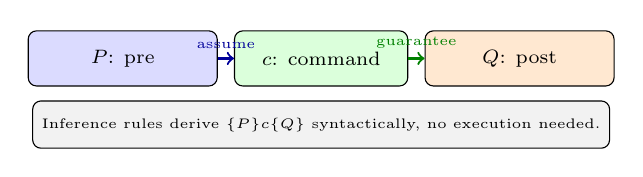
\begin{tikzpicture}[scale=0.84,every node/.style={font=\scriptsize}]
  \node[draw,fill=blue!14,rounded corners=3pt,minimum width=2.4cm,minimum height=0.7cm,align=center] (p) at (-3.0,0) {$P$: pre};
  \node[draw,fill=green!14,rounded corners=3pt,minimum width=2.2cm,minimum height=0.7cm,align=center] (c) at (0,0) {$c$: command};
  \node[draw,fill=orange!18,rounded corners=3pt,minimum width=2.4cm,minimum height=0.7cm,align=center] (q) at (3.0,0) {$Q$: post};
  \draw[->,thick,blue!60!black] (p) -- (c) node[midway,above,font=\tiny] {assume};
  \draw[->,thick,green!50!black] (c) -- (q) node[midway,above,font=\tiny] {guarantee};
  \node[draw,fill=gray!10,rounded corners=3pt,minimum width=5.4cm,minimum height=0.6cm,align=center,font=\tiny] at (0,-1.0) {Inference rules derive $\{P\}c\{Q\}$ syntactically, no execution needed.};
\end{tikzpicture}
\caption{Hoare triple intuition: $P$ is what we need on entry, $Q$ is what we get on exit if $c$ terminates. Rules let us compose triples for larger programs.}
\label{fig:hoare-intuition}
\end{figure}

Key rules (with $P[e/x]$ meaning $P$ with $x$ replaced by $e$):

\begin{center}
\small
\begin{tabular}{cl}
\toprule
Rule & Schema \\
\midrule
Assignment & $\{P[e/x]\}~x:=e~\{P\}$ \\
Sequence & $\frac{\{P\}c_1\{R\}\quad \{R\}c_2\{Q\}}{\{P\}c_1;c_2\{Q\}}$ \\
Conditional & $\frac{\{P\land b\}c_1\{Q\}\quad \{P\land \neg b\}c_2\{Q\}}{\{P\}\texttt{if }b\texttt{ then }c_1\texttt{ else }c_2\{Q\}}$ \\
While & $\frac{\{I\land b\}c\{I\}}{\{I\}\texttt{while }b\texttt{ do }c\{I\land \neg b\}}$ where $I$ is the invariant \\
Consequence & $\frac{P\Rightarrow P'\quad \{P'\}c\{Q'\}\quad Q'\Rightarrow Q}{\{P\}c\{Q\}}$ \\
\bottomrule
\end{tabular}
\end{center}

\begin{example}[While with invariant]
Program to sum $0$..$n$: \texttt{s:=0; i:=0; while i<=n do \{ s:=s+i; i:=i+1 \}}. Invariant $I: s=\sum_{k=0}^{i-1}k \land 0\le i\le n+1$. Show $\{I\land i\le n\}~body~\{I\}$ by assignment rule, then while rule gives $\{I\}loop\{I\land i>n\}$, which implies $s=n(n+1)/2$.
\end{example}

\begin{lstlisting}[language=Python]
# Hoare-style assertion as runtime check (testing vs. proving)
def sum_to_n(n):
    s, i = 0, 0
    # invariant: s == i*(i-1)//2  and  0 <= i <= n+1
    while i <= n:
        assert s == i*(i-1)//2  # would be discharged by a verifier
        s += i; i += 1
    assert s == n*(n+1)//2
    return s
\end{lstlisting}

Finding invariants is the creative step; templates (\texttt{x == c}, \texttt{x \\le y}, \texttt{a[i] < N}) and counterexample-guided inference help. Tools like Dafny, Frama-C and Verus automate the bookkeeping once you supply annotations, while Infer and CodeQL sacrifice completeness for speed on million-line codebases.

 checkers (Dafny, Frama-C) automate the bookkeeping once you supply them.

% ============================================================
\section{Model Checking: Exhausting the State Space}
\label{sec:model-checking}
Hoare logic is compositional but manual. Model checking is automatic: given a finite-state model $M$ and a temporal property $\phi$ (e.g., ``no execution reaches a state where both threads hold the same lock''), exhaustively explore all reachable states and verify $\phi$.

\begin{definition}[Model checking]
Let $M=(S,S_0,R,L)$ be a Kripke structure ($S$ states, $R\subseteq S\times S$ transitions). Model checking decides $M\models\phi$ where $\phi$ is in LTL/CTL (e.g., $\mathbf{G}\neg\text{error}$, $\mathbf{AG}(req\to \mathbf{AF}resp)$). If violated, a counterexample trace is produced.
\end{definition}

\begin{figure}[h]\centering
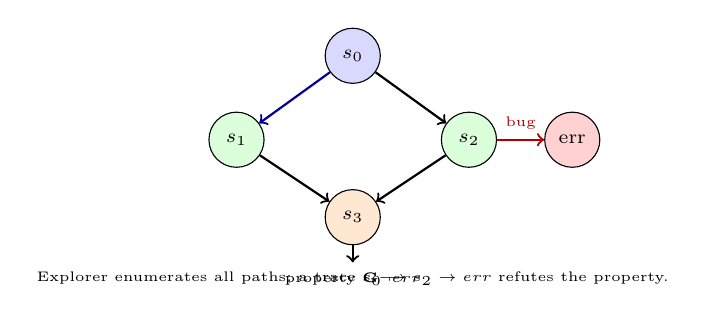
\begin{tikzpicture}[scale=0.82,every node/.style={font=\scriptsize}]
  \node[draw,circle,fill=blue!15,minimum size=0.7cm] (s0) at (0,1.6) {$s_0$};
  \node[draw,circle,fill=green!14,minimum size=0.7cm] (s1) at (-1.8,0.3) {$s_1$};
  \node[draw,circle,fill=green!14,minimum size=0.7cm] (s2) at (1.8,0.3) {$s_2$};
  \node[draw,circle,fill=orange!18,minimum size=0.7cm] (s3) at (0,-0.9) {$s_3$};
  \node[draw,circle,fill=red!18,minimum size=0.7cm] (err) at (3.4,0.3) {err};
  \draw[->,thick,blue!60!black] (s0) -- (s1); \draw[->,thick] (s0) -- (s2);
  \draw[->,thick] (s1) -- (s3); \draw[->,thick] (s2) -- (s3);
  \draw[->,thick,red!70!black] (s2) -- (err) node[midway,above,font=\tiny] {bug};
  \draw[->,thick] (s3) -- ++(0,-0.7) node[below,font=\tiny] {property $\mathbf{G}\neg err$};
  \node[font=\tiny,align=center] at (0,-1.85) {Explorer enumerates all paths; a trace $s_0\to s_2\to err$ refutes the property.};
\end{tikzpicture}
\caption{Model checking explores the reachable state graph. If the error state is reachable, the checker returns the witnessing trace; otherwise the property holds for the model (not necessarily the real code).}
\label{fig:model-checking}
\end{figure}

State explosion is the enemy: $n$ boolean variables give $2^n$ states; a 32-bit integer already has $2^{32}$ values. Mitigations include symbolic model checking (BDDs, SAT/SMT), bounded checking (up to $k$ steps, as in CBMC), $k$-induction, abstraction (predicate/CEGAR), and compositional reasoning that verifies modules in isolation.

 $n$ boolean variables give $2^n$ states. Mitigations include symbolic model checking (BDDs, SAT/SMT), bounded checking (up to $k$ steps, as in CBMC), abstraction (predicate/CEGAR), and compositional reasoning.

\begin{lstlisting}[language=C]
// CBMC bounded model checking example (checks assert for all inputs up to bound)
#include <assert.h>
int max(int a, int b){ return (a>b)?a:b; }
int main(){
    int x = nondet_int(), y = nondet_int();
    int m = max(x,y);
    assert(m >= x && m >= y);       // CBMC proves this holds
    // assert(m == x || m == y);    // also holds; try and see the proof
}
\end{lstlisting}

% ============================================================
\section{Taint Analysis: Tracking Untrusted Data}
\label{sec:taint}
Security properties are often about flow: ``untrusted input never reaches a sensitive sink without sanitization.'' Taint analysis tracks this as a data-flow problem.

\begin{definition}[Taint analysis]
Label values as \emph{tainted} (attacker-controlled) or \emph{clean}. Sources introduce taint (user input, file read, network recv). Propagation rules carry taint through assignments and operations (e.g., $y:=x$ taints $y$ if $x$ is tainted). Sinks (SQL query, \texttt{innerHTML}, \texttt{exec}) must not receive tainted data unless a \emph{sanitizer} (encoder, parameteriser) cleaned it. A path source $\twoheadrightarrow$ sink without sanitizer is a vulnerability.
\end{definition}

\begin{figure}[h]\centering
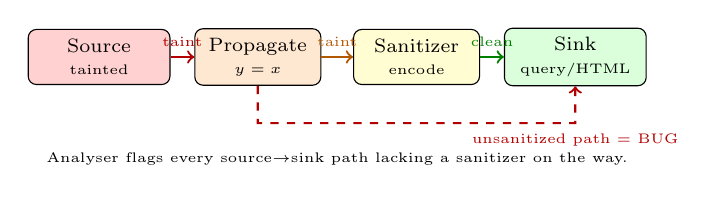
\begin{tikzpicture}[scale=0.84,every node/.style={font=\scriptsize}]
  \node[draw,fill=red!18,rounded corners=3pt,minimum width=1.8cm,minimum height=0.7cm,align=center] (src) at (-3.6,0) {Source\\ \tiny tainted};
  \node[draw,fill=orange!18,rounded corners=3pt,minimum width=1.6cm,minimum height=0.7cm,align=center] (prop) at (-1.2,0) {Propagate\\ \tiny $y=x$};
  \node[draw,fill=yellow!18,rounded corners=3pt,minimum width=1.6cm,minimum height=0.7cm,align=center] (san) at (1.2,0) {Sanitizer\\ \tiny encode};
  \node[draw,fill=green!14,rounded corners=3pt,minimum width=1.8cm,minimum height=0.7cm,align=center] (sink) at (3.6,0) {Sink\\ \tiny query/HTML};
  \draw[->,thick,red!70!black] (src) -- (prop) node[midway,above,font=\tiny] {taint};
  \draw[->,thick,orange!70!black] (prop) -- (san) node[midway,above,font=\tiny] {taint};
  \draw[->,thick,green!50!black] (san) -- (sink) node[midway,above,font=\tiny] {clean};
  \draw[->,thick,red!70!black,dashed] (prop) -- ++(0,-1.0) -| (sink) node[midway,below,font=\tiny] {unsanitized path = BUG};
  \node[font=\tiny,align=center] at (0,-1.55) {Analyser flags every source$\to$sink path lacking a sanitizer on the way.};
\end{tikzpicture}
\caption{Taint flow: sources inject taint, propagation carries it, sanitizers remove it, sinks must not receive tainted data. A path that bypasses sanitization is reported.}
\label{fig:taint}
\end{figure}

Analysis may be \emph{sound} (every reported bug is real, but some bugs missed if analysis over-approximates sanitizers) or \emph{complete} (every bug found, but false positives). Practical tools (CodeQL, Semgrep, Infer) tune for low false positives on the bug classes that matter (XSS, SQLi, path traversal) and integrate into CI.

\begin{remark}[Limits of verification]
Verification proves a stated property of a model, not ``the program is secure.'' A wrong spec, a missed source/sink, or a gap between model and hardware (e.g., Spectre) leaves real bugs unproven. Pair verification with fuzzing and code review: prove what you can, test the rest, and monitor the gap.
\end{remark}

% ============================================================
\section{From Hoare to Automation: VCGen}
\label{sec:vcgen}
Hoare rules are syntax-directed; verification-condition generation (VCGen) applies them mechanically to produce a logical formula whose validity implies the triple. An SMT solver (Z3, CVC5) discharges the formula. The human supplies loop invariants and procedure contracts; the tool checks that every path respects them. This is the engine behind Dafny, Why3 and Frama-C WP: the program is correct iff the generated VCs are all valid.

% ============================================================
\section{Abstract Interpretation and Soundness}
\label{sec:abstract}
Many analysers do not prove a single property but over-approximate all behaviours via \emph{abstract interpretation}: map concrete states to an abstract domain (e.g., intervals, taint labels) and compute a fixpoint that covers every execution. If the abstract fixpoint has no error, the concrete program has none (sound). If it reports an error, it may be a false positive (incomplete) because the abstraction was too coarse.

Widening accelerates fixpoint convergence at the cost of precision; narrowing recovers some. The art is choosing a domain precise enough for the property (e.g., intervals for array bounds, octagons for relations, taint for injection) yet cheap enough to run on a million-line codebase in CI. Counterexample-guided abstraction refinement (CEGAR) starts coarse and refines only where a spurious counterexample requires it.

 convergence at the cost of precision; narrowing recovers some. The art is choosing a domain precise enough for the property (e.g., intervals for array bounds, taint for injection) yet cheap enough to run on a million-line codebase in CI.

\begin{remark}[Bug-finding vs.\ verification]
Static analysers span a spectrum: unsound bug-finders (fast, many false negatives but few false positives, e.g., linting) vs.\ sound verifiers (slow, no false negatives but many false positives). For security, soundness for the target bug class (injection, overflow) is preferred even if it means triaging noise; for productivity, precision wins.
\end{remark}


\begin{remark}[Choosing a property]
Start with the property that matters most: memory safety for C/C++, injection freedom for web code, or functional correctness for a key derivation. A narrow, precisely stated property that the team can keep green in CI beats a broad, aspirational spec that is always red.
\end{remark}


\begin{example}[Taint in CI]
CodeQL query: \texttt{from Source s, Sink k where s.flowsTo(k) and not exists Sanitizer n | n.between(s,k) select k, "tainted flow"}. Landing this query in CI and annotating sanitizers (e.g., \texttt{htmlEscape}) turns a class of vulnerabilities into a build break rather than a post-release patch.
\end{example}


\begin{remark}[Scaling to the codebase]
Whole-program verification does not scale; compositional verification does. Verify critical modules (crypto, parsers, access control) with strong specs, and cover the rest with taint analysis and fuzzing. The report that matters is ``which modules are verified for which properties,'' not ``is the whole program verified.''
\end{remark}

% ============================================================
\section{Exercises}
\label{sec:ch06-exercises}
\begin{enumerate}[label=E6.\arabic*, leftmargin=*, itemsep=0.6em]
    \item \textbf{Hoare derivation.} Prove $\{x=n\}~y:=0;~while~x>0~do~\{y:=y+x;~x:=x-1\}~\{y=n(n+1)/2\}$ by giving invariant $I$ and showing each rule application. State where the consequence rule is used.
    \item \textbf{Model checking bound.} A program has 20 boolean state bits and a bug at depth 15. How many states in the worst case? Why does bounded checking to $k=10$ miss it? What abstraction could make it visible without exploring $2^{20}$ states?
    \item \textbf{Taint spec.} For a web app, list two sources, two sinks and one sanitizer for each of (a) SQLi and (b) XSS. Draw a taint graph with one clean and one buggy path for each, and explain why string concatenation is still flagged even if a filter removes \texttt{<script>}.
    \item \textbf{Soundness vs.\ precision.} A taint analyser flags every \texttt{query = "..." + input} as SQLi (sound but imprecise). How would you reduce false positives without losing soundness? Discuss allow-listing sanitizers vs.\ demand-driven analysis.
    \item \textbf{Invariant inference.} Why is loop invariant inference undecidable in general? Give a loop where a human sees the invariant instantly but a simple analyser fails, and suggest an annotation or abstract domain that would help.
\end{enumerate}

\section*{Chapter Notes}
Hoare logic from Hoare (1969); separation logic (Reynolds, O'Hearn) extends it to heaps. Model checking is Clarke \& Emerson and Sifakis (Turing Award 2007); SPIN (Holzmann), CBMC (Clarke et al.), and TLA+ (Lamport) are canonical tools. Taint analysis foundations in Volpano et al. and Livshits \& Lam (2005); CodeQL, Infer and Semgrep are modern incarnations. Soundness/completeness trade-offs surveyed in Chess \& McGraw.

% End of Chapter 6
